% p1-chp03-parser.tex

\chapter{Syntax Analysis and the Parser}
\label{chp:parser}

The parser is the second phase of a compiler. It reads the token stream
produced by the lexer and builds a parse tree according to the grammar,
checking along the way that the tokens form a program that the grammar
allows. This chapter gives OctaC's grammar, in LL(1) form, and describes
the recursive descent parser built from it. The parser
chooses a production from one token of lookahead, builds the tree as it
goes, and recovers when it hits a syntax error. The source code of the
parser is available at:
\url{https://github.com/Octa-C/compiler/tree/main/parser}

\section{Grammar Theory}
\label{sec:grammar-theory}

\subsection{Left-Recursive Grammars}

A grammar is left recursive if it has a nonterminal $A$ with a production
of the form $A \to A\alpha \mid \beta$, where $\beta$ does not itself start
with $A$. Such a rule can never be used by a recursive descent parser: the
function for $A$ would call itself before reading any token, and never
terminate \cite{aho2006compilers}. The standard fix moves the recursive
part into a new nonterminal $A'$ that follows the non-recursive
alternative:
\begin{center}
$A \to \beta A'$ \qquad $A' \to \alpha A' \mid \varepsilon$
\end{center}
This produces the same language as the original rule, since $A$ is still
$\beta$ followed by zero or more repetitions of $\alpha$, just written so
that the recursion is no longer on the left \cite{aho2006compilers}. A sum
written as a left-recursive grammar, for example,
\begin{center}
$G \to G \mathbin{+} T \mid T$
\end{center}
rewrites the same way, with $\beta$ as $T$ and $\alpha$ as $\mathbin{+}\, T$:
\begin{center}
$G \to T G'$ \qquad $G' \to \mathbin{+}\, T G' \mid \varepsilon$
\end{center}

A grammar also needs left factoring when two productions of the same
nonterminal share a prefix, so that the parser cannot tell them apart from
the first token. Two productions of the form $A \to \alpha\beta_1 \mid
\alpha\beta_2$ can be rewritten by factoring the shared prefix out into a
new nonterminal, deferring the choice between $\beta_1$ and $\beta_2$ until
after $\alpha$ has been read \cite{aho2006compilers}:
\begin{center}
$A \to \alpha A'$ \qquad $A' \to \beta_1 \mid \beta_2$
\end{center}
A statement grammar with three productions that all start with an
identifier,
\begin{center}
$S \to \texttt{id}\ \texttt{=}\ \texttt{number} \mid \texttt{id}\,\texttt{(}\texttt{)}
\mid \texttt{id}\,\texttt{[}\texttt{]}$
\end{center}
needs exactly this treatment: factoring \texttt{id} out of all three gives
$S \to \texttt{id}\,S'$, with $S'$ then choosing between the three endings:
\begin{center}
$S \to \texttt{id}\,S'$ \qquad
$S' \to \texttt{=}\ \texttt{number} \mid \texttt{(}\texttt{)} \mid \texttt{[}\texttt{]}$
\end{center}

\subsection{LL(k) Grammars}

Eliminating left recursion and left factoring, as above, is not just a fix
for recursive descent specifically: it is what turns a grammar into a
grammar of a well known class. A parser that reads its input left to right
and builds a leftmost derivation, choosing a production for each
nonterminal from the next $k$ tokens of input without ever backtracking, is
called an LL($k$) parser, and a grammar it can parse this way is an LL($k$)
grammar \cite{aho2006compilers}. The first L is the direction the input is
read, the second is the kind of derivation built, and $k$ is how far ahead
the parser is allowed to look.

A grammar fails to be LL(1) when some nonterminal has two productions whose
possible starting tokens overlap, since then one token of lookahead is not
enough to choose between them \cite{aho2006compilers}. That is precisely
the problem left recursion and shared prefixes cause, and precisely what
eliminating them fixes. LL(1), with a single token of lookahead, is the
common case, and it is exactly what a recursive descent parser gives for
free: each nonterminal's function can look at one token and immediately
know which production to take.

\section{The Grammar}

\subsection{Notation}

Nonterminals are written in \nt{italics}. A keyword, or a token with
several lexemes, is written in capitals, as its token name: \stok{FUNCTION}
for the keyword \code{function}, \stok{SCALAR} for a type name such as
\code{i32}. A token that is a single fixed symbol, such as \texttt{\{} or
\texttt{->}, is written as that symbol. Three tokens are shortened for
readability: an identifier is written \texttt{ID} rather than
\stok{IDENTIFIER}, an assignment is written \texttt{=} rather than
\stok{ASSIGNMENT}, and the end of input is written \texttt{\$} rather than
\stok{COMPILER\_EOF}. $\varepsilon$ is the empty string, and \nt{Program}
is the start symbol.

The grammar that follows is OctaC's grammar in LL(1) form, rewritten by
the two transformations of Section~\ref{sec:grammar-theory}. A sum, for
example, was left recursive: \nt{Sum} $\to$ \nt{Sum} \stok{PLUSMINUS}
\nt{Product} $\mid$ \nt{Product} became \nt{Sum} $\to$ \nt{Product}
\nt{Sum}$'$, \nt{Sum}$'$ $\to$ \stok{PLUSMINUS} \nt{Product} \nt{Sum}$'$
$\mid$ $\varepsilon$. And \nt{Stmt} needed left factoring: a statement
starting with an identifier might be an assignment, an indexed
assignment, or a function call, and the parser cannot know which until it
has read past the identifier, so factoring that identifier out gives
\nt{Stmt} $\to$ \texttt{ID} \nt{Stmt}$'$, with \nt{Stmt}$'$ then branching
on whatever token follows. The grammar is grouped the way the parser's
source code groups its functions: the program and its functions, types,
statements, and expressions.

\subsection{Program and Functions}

A program is one or more functions, each with a parameter list, a return
type, and a body. \nt{Params} is empty for a function with no parameters,
and \nt{ParamList} is a comma separated list of a type and a name, with no
trailing comma.

{\small
\renewcommand{\arraystretch}{1.3}
\begin{longtable}{@{}>{\raggedright\arraybackslash}p{70pt} p{0.80\linewidth}@{}}
\nt{Program} & $\to$ \stok{FUNCTION} \texttt{ID} \texttt{(} \nt{Params} \texttt{)} \texttt{->} \nt{Type} \texttt{\{} \nt{Stmts} \texttt{\}} \nt{Program}$'$ \\
\nt{Program}$'$ & $\to$ \stok{FUNCTION} \texttt{ID} \texttt{(} \nt{Params} \texttt{)} \texttt{->} \nt{Type} \texttt{\{} \nt{Stmts} \texttt{\}} \nt{Program}$'$ $\mid$ $\varepsilon$ \\
\nt{Params} & $\to$ \nt{ParamList} $\mid$ $\varepsilon$ \\
\nt{ParamList} & $\to$ \nt{Type} \texttt{ID} \nt{ParamList}$'$ \\
\nt{ParamList}$'$ & $\to$ \texttt{,} \nt{Type} \texttt{ID} \nt{ParamList}$'$ $\mid$ $\varepsilon$ \\
\end{longtable}}

\subsection{Types}

A type is a scalar type, \code{string}, or a \code{vector} or \code{matrix}
parameterized by an element type and, optionally, its dimensions. The
dimensions are themselves omitted when a declaration's shape can be
inferred from its initializer, which is a semantic rule checked after
parsing rather than one the grammar enforces.

{\small
\renewcommand{\arraystretch}{1.3}
\begin{longtable}{@{}>{\raggedright\arraybackslash}p{70pt} p{0.80\linewidth}@{}}
\nt{Type} & $\to$ \stok{SCALAR} \newline
  $\mid$ \stok{STRING} \newline
  $\mid$ \stok{VECTOR} \texttt{<} \stok{SCALAR} \nt{Type}$'$ \newline
  $\mid$ \stok{MATRIX} \texttt{<} \stok{SCALAR} \nt{Type}$''$ \\
\nt{Type}$'$ & $\to$ \texttt{>} $\mid$ \texttt{,} \stok{INT} \texttt{>} \\
\nt{Type}$''$ & $\to$ \texttt{>} $\mid$ \texttt{,} \stok{INT} \texttt{,} \stok{INT} \texttt{>} \\
\end{longtable}}

\subsection{Statements}

Every kind of statement in Chapter~\ref{chp:introduction} has its own
production here. \nt{Stmt}$'$ resolves what follows an identifier: an
assignment, an indexed assignment or an indexed compound target, or a
function call. \nt{Stmt}$'''$ resolves the two forms of \code{for}, the
range form and the \code{for\ldots in} form, from the single token that
follows the loop variable's name. \nt{CaseVal} restricts a \code{case}
label to a literal, optionally signed for a number, which keeps
\code{caseof} to constant labels rather than arbitrary expressions.

{\small
\renewcommand{\arraystretch}{1.3}
\begin{longtable}{@{}>{\raggedright\arraybackslash}p{70pt} p{0.80\linewidth}@{}}
\nt{Stmts} & $\to$ \nt{Stmts}$'$ \\
\nt{Stmts}$'$ & $\to$ \nt{Stmt} \nt{Stmts}$'$ $\mid$ $\varepsilon$ \\
\nt{Stmt} & $\to$ \nt{Type} \texttt{ID} \texttt{=} \nt{Expr} \texttt{;} \newline
  $\mid$ \texttt{ID} \nt{Stmt}$'$ \newline
  $\mid$ \stok{IF} \texttt{(} \nt{Expr} \texttt{)} \texttt{\{} \nt{Stmts} \texttt{\}} \nt{ElseIfs} \nt{Stmt}$''$ \newline
  $\mid$ \stok{FOR} \texttt{(} \nt{Type} \texttt{ID} \nt{Stmt}$'''$ \newline
  $\mid$ \stok{UNTIL} \texttt{(} \nt{Expr} \texttt{)} \texttt{\{} \nt{Stmts} \texttt{\}} \newline
  $\mid$ \stok{DO} \texttt{\{} \nt{Stmts} \texttt{\}} \stok{UNTIL} \texttt{(} \nt{Expr} \texttt{)} \texttt{;} \newline
  $\mid$ \stok{CASEOF} \texttt{(} \nt{Expr} \texttt{)} \texttt{\{} \nt{Cases} \nt{Stmt}$''''$ \newline
  $\mid$ \stok{RETURN} \nt{Expr} \texttt{;} \newline
  $\mid$ \stok{BREAK} \texttt{;} \newline
  $\mid$ \stok{CONTINUE} \texttt{;} \\
\nt{Stmt}$'$ & $\to$ \texttt{=} \nt{Expr} \texttt{;} $\mid$ \texttt{[} \nt{Expr} \texttt{]} \nt{Stmt}$'''''$ $\mid$ \texttt{(} \nt{Args} \texttt{)} \texttt{;} \\
\nt{Stmt}$''$ & $\to$ \stok{ELSE} \texttt{\{} \nt{Stmts} \texttt{\}} $\mid$ $\varepsilon$ \\
\nt{Stmt}$'''$ & $\to$ \texttt{=} \nt{Expr} \texttt{...} \nt{Expr} \texttt{)} \texttt{\{} \nt{Stmts} \texttt{\}} $\mid$ \stok{IN} \nt{Expr} \texttt{)} \texttt{\{} \nt{Stmts} \texttt{\}} \\
\nt{Stmt}$''''$ & $\to$ \texttt{\}} $\mid$ \stok{DEFAULT} \texttt{:} \nt{Stmts} \texttt{\}} \\
\nt{Stmt}$'''''$ & $\to$ \texttt{=} \nt{Expr} \texttt{;} $\mid$ \texttt{[} \nt{Expr} \texttt{]} \texttt{=} \nt{Expr} \texttt{;} \\
\nt{ElseIfs} & $\to$ \nt{ElseIfs}$'$ \\
\nt{ElseIfs}$'$ & $\to$ \stok{ELSEIF} \texttt{(} \nt{Expr} \texttt{)} \texttt{\{} \nt{Stmts} \texttt{\}} \nt{ElseIfs}$'$ $\mid$ $\varepsilon$ \\
\nt{Cases} & $\to$ \nt{Cases}$'$ \\
\nt{Cases}$'$ & $\to$ \stok{CASE} \nt{CaseVal} \texttt{:} \nt{Stmts} \nt{Cases}$'$ $\mid$ $\varepsilon$ \\
\nt{CaseVal} & $\to$ \stok{INT} $\mid$ \stok{FLOAT} $\mid$ \stok{STRING_LIT} $\mid$ \stok{BOOL_LIT} $\mid$ \stok{PLUSMINUS} \nt{CaseVal}$'$ \\
\nt{CaseVal}$'$ & $\to$ \stok{INT} $\mid$ \stok{FLOAT} \\
\end{longtable}}

\subsection{Expressions}
\label{sec:expr-grammar}

OctaC resolves operator precedence the usual way a recursive descent
grammar does: as a chain of nonterminals, one per precedence level, each
built from the next one down. Table~\ref{tab:precedence} lists the chain
from loosest to tightest. Climbing down it is how the grammar encodes
precedence without parentheses: a \nt{Sum} is built from \nt{Product}s, so
a product never has to yield to a sum that has not finished, and
\code{1 + 2 * 3} is parsed with the multiplication nested inside the
addition rather than the other way around.

{\small
\renewcommand{\arraystretch}{1.2}
\begin{longtable}{@{}cll@{}}
\caption{Precedence levels of OctaC's operators.}
\label{tab:precedence} \\
\toprule
\textbf{Level} & \textbf{Nonterminal} & \textbf{Operators} \\
\midrule
\endfirsthead
\toprule
\textbf{Level} & \textbf{Nonterminal} & \textbf{Operators} \\
\midrule
\endhead
1 (loosest) & \nt{Expr} & \code{or} \\
2 & \nt{AndExpr} & \code{and} \\
3 & \nt{NotExpr} & \code{not} \\
4 & \nt{Comp} & \texttt{<} \texttt{>} \texttt{<=} \texttt{>=} \code{is} \code{is not} \\
5 & \nt{Sum} & \texttt{+} \texttt{-} \\
6 & \nt{Product} & \texttt{*} \texttt{/} \texttt{\%} \texttt{.*} \texttt{./} \\
7 & \nt{Operand} & unary \texttt{+} \texttt{-} \\
8 & \nt{IndexedData} & \texttt{\textquotesingle{}} (transpose), \texttt{[} \nt{Expr} \texttt{]} (indexing) \\
9 (tightest) & \nt{Data} & literals, identifiers, calls, \texttt{(} \nt{Expr} \texttt{)}, \texttt{[} \nt{Args} \texttt{]} \\
\bottomrule
\end{longtable}}

\nt{Comp}$''$ exists because \code{is not} is two tokens where every other
comparison is one: after \code{is}, a \stok{NOT} token means \code{is not}
and anything else in FIRST(\nt{Sum}) means a plain \code{is}, which is
exactly the one token of lookahead the grammar is allowed.

{\small
\renewcommand{\arraystretch}{1.3}
\begin{longtable}{@{}>{\raggedright\arraybackslash}p{70pt} p{0.80\linewidth}@{}}
\nt{Expr} & $\to$ \nt{AndExpr} \nt{Expr}$'$ \\
\nt{Expr}$'$ & $\to$ \stok{OR} \nt{AndExpr} \nt{Expr}$'$ $\mid$ $\varepsilon$ \\
\nt{AndExpr} & $\to$ \nt{NotExpr} \nt{AndExpr}$'$ \\
\nt{AndExpr}$'$ & $\to$ \stok{AND} \nt{NotExpr} \nt{AndExpr}$'$ $\mid$ $\varepsilon$ \\
\nt{NotExpr} & $\to$ \stok{NOT} \nt{NotExpr} $\mid$ \nt{Comp} \\
\nt{Comp} & $\to$ \nt{Sum} \nt{Comp}$'$ \\
\nt{Comp}$'$ & $\to$ \texttt{<} \nt{Sum} $\mid$ \texttt{>} \nt{Sum} $\mid$ \texttt{<=} \nt{Sum} $\mid$ \texttt{>=} \nt{Sum} $\mid$ \stok{IS} \nt{Comp}$''$ $\mid$ $\varepsilon$ \\
\nt{Comp}$''$ & $\to$ \nt{Sum} $\mid$ \stok{NOT} \nt{Sum} \\
\nt{Sum} & $\to$ \nt{Product} \nt{Sum}$'$ \\
\nt{Sum}$'$ & $\to$ \stok{PLUSMINUS} \nt{Product} \nt{Sum}$'$ $\mid$ $\varepsilon$ \\
\nt{Product} & $\to$ \nt{Operand} \nt{Product}$'$ \\
\nt{Product}$'$ & $\to$ \stok{STAR_SLASH_MOD} \nt{Operand} \nt{Product}$'$ \newline
  $\mid$ \texttt{.*} \nt{Operand} \nt{Product}$'$ \newline
  $\mid$ \texttt{./} \nt{Operand} \nt{Product}$'$ \newline
  $\mid$ $\varepsilon$ \\
\nt{Operand} & $\to$ \stok{PLUSMINUS} \nt{Operand} $\mid$ \nt{IndexedData} \\
\nt{IndexedData} & $\to$ \nt{Data} \nt{IndexedData}$'$ \\
\nt{IndexedData}$'$ & $\to$ \texttt{\textquotesingle{}} \nt{IndexedData}$'$ $\mid$ \texttt{[} \nt{Expr} \texttt{]} \nt{IndexedData}$'$ $\mid$ $\varepsilon$ \\
\nt{Data} & $\to$ \texttt{ID} \nt{Data}$'$ \newline
  $\mid$ \stok{INT} \newline
  $\mid$ \stok{FLOAT} \newline
  $\mid$ \stok{STRING_LIT} \newline
  $\mid$ \stok{BOOL_LIT} \newline
  $\mid$ \texttt{(} \nt{Expr} \texttt{)} \newline
  $\mid$ \texttt{[} \nt{Args} \texttt{]} \\
\nt{Data}$'$ & $\to$ \texttt{(} \nt{Args} \texttt{)} $\mid$ $\varepsilon$ \\
\nt{Args} & $\to$ \nt{ArgList} $\mid$ $\varepsilon$ \\
\nt{ArgList} & $\to$ \nt{Expr} \nt{ArgList}$'$ \\
\nt{ArgList}$'$ & $\to$ \texttt{,} \nt{Expr} \nt{ArgList}$'$ $\mid$ $\varepsilon$ \\
\end{longtable}}

\section{How the Parser Works}

The parser is a recursive descent parser over the grammar above, built
around a single invariant: because the grammar is LL(1), the next token
always picks exactly one production, so no nonterminal's function ever has
to guess or back up \cite{aho2006compilers}.

\subsection{One Function per Nonterminal}

Every nonterminal in the grammar has its own function. Each function looks
at the next token, chooses the one production it matches, and calls the
functions for the nonterminals on that production's right-hand side in
order, building a tree node as it goes. An empty production is taken
whenever the next token does not start the non-empty one, which is always
decidable from one token because the grammar is LL(1).

\begin{lstlisting}[style=pseudocode,
    caption={The function behind \nt{Data}.}, label=lst:data]
function data():
    node <- new node(Data)
    switch next.type:
        case ID:
            node.children += shift()
            node.children += dataP()
        case INT:
        case FLOAT:
        case STRING_LIT:
        case BOOL_LIT:
            node.children += shift()
        case LPAREN:
            node.children += shift()
            node.children += expr()
            node.children += expect(RPAREN)
        case LBRACKET:
            node.children += shift()
            node.children += args()
            node.children += expect(RBRACKET)
        default:
            reportExpected("an expression")
            throw SyntaxError
    return node
\end{lstlisting}

Listing~\ref{lst:data} shows this for \nt{Data}: the \code{switch} on the
next token's type is exactly the one token of lookahead the grammar's
LL(1) property guarantees is enough to pick a case. Read against
Section~\ref{sec:lexer-algorithm}'s scanning loop, the shape is the same
idea one level up: where the lexer's loop walks a table one character at a
time, the parser's recursion walks the grammar one symbol at a time.

\subsection{Matching Terminals}

A terminal is matched with \code{expect(type)}, which consumes the next
token if it has the required type and reports a syntax error otherwise,
or \code{shift()}, which consumes a token already known to be there,
such as inside a \code{switch} on the next token's type. Both add the
consumed token to the current node as a leaf.

\subsection{Building the Tree}

A node is either a nonterminal, with one child per symbol of the
production that derived it, or a leaf holding the token that matched a
terminal. A nonterminal with no children derived the empty string, and is
written \code{(empty)} when the tree is printed. The tree is printed one
node per line, indented two spaces per level: a nonterminal as its name
from the grammar, with each prime written \code{P} and the count of primes
from two upward (\nt{Stmt}$'$ is \code{StmtP}, \nt{Stmt}$''$ is
\code{StmtP2}), and a leaf as its token, in the same \code{<TYPE, value>}
form the lexer uses. Where the lexer rewinds to the last accepting state on
a dead end, the parser recovers to the next point the grammar can resume
from, described next.

\section{Errors and Recovery}

A syntax error is reported the same way a lexical error is: to the
standard error stream, with the line and column, the source line, and a
marker under the offending text. The message names what the grammar
allowed at that point and what was found instead:

\begin{lstlisting}[style=pseudocode]
main.oc:2:13: error: expected an expression but found ';'
 2 |     i32 x = ;
   |             ^
\end{lstlisting}

\subsection{Recovery}

Reporting an error throws, which unwinds to the nearest recovery point
rather than to the top of the parse. Two recovery points exist, matching
the two places a broken construct can be skipped without losing track of
where the rest of the program begins.

\begin{itemize}
    \item \textbf{Inside a block.} A broken statement is skipped up to the
    next \code{;} at the same brace depth it started at, or to the \code{\}}
    that closes a block the statement itself opened, whichever comes
    first. A count of unmatched \code{\{} against \code{\}} is kept
    throughout, so skipping never mistakes a brace that belongs to a
    nested block for the one that closes the enclosing one.
    \item \textbf{Between functions.} A broken function, or a broken
    top-level construct, is skipped up to the next \stok{FUNCTION}
    keyword, or to the end of input.
\end{itemize}

Because recovery always lands on a token that can start a new statement, a
new function, \code{case}, or \code{default}, parsing carries on from
there rather than stopping at the first error. One run can therefore
report many syntax errors in a file, the same way one run of the lexer
reports many lexical errors. Two errors reported at the same token are
collapsed into one, since a single bad token otherwise tends to be rejected
by more than one function on the way back up. No tree is produced for a
file that had any syntax error, even though the recovered parse continues
to the end of the input to keep finding them. Table~\ref{tab:parser-errors} shows 
some invalid inputs and the diagnostic each one produces.

\begin{table}[H]
\centering
\small
\renewcommand{\arraystretch}{1.3}
\begin{tabular}{@{}>{\raggedright\arraybackslash}p{150pt}>{\raggedright\arraybackslash}p{0.62\linewidth}@{}}
\toprule
\textbf{Input} & \textbf{Diagnostic} \\
\midrule
\texttt{i32 x = ;} & \texttt{expected an expression but found ';'} \\
\texttt{function -> i32 \{} & \texttt{expected an identifier but found '->'} \\
\texttt{for (i32 i 0...1) \{} & \texttt{expected an assignment operator or 'in' but found '0'} \\
\texttt{matrix<f32, 2> m = 1;} & \texttt{expected ',' but found '>'} \\
\bottomrule
\end{tabular}
\caption{Examples of syntax errors.}
\label{tab:parser-errors}
\end{table}

A file that ends with an unclosed \code{if} shows recovery reaching the end
of input rather than a token: since no \code{\}} ever arrives to skip to,
the error is reported once, at the end of input, rather than repeated for
every nesting level left open.

\begin{lstlisting}[style=pseudocode]
    if (x) {
        y = 1;
(end of input)
\end{lstlisting}

\begin{sloppypar}
This produces a single diagnostic, \texttt{4:1: expected '\}' but found end
of input}.
\end{sloppypar}

\section{Sample Parses}

\subsection{A Minimal Program}

A short, complete OctaC program is a single function that returns
immediately:

\begin{lstlisting}
function main() -> i32 {
    return 0;
}
\end{lstlisting}

Even this short a program produces a deep tree, because every expression,
here just the literal \code{0}, passes through the full precedence chain
of Section~\ref{sec:expr-grammar} on its way down to \nt{Data}. Listing~
\ref{lst:tiny-tree} is the tree \code{--emit-parse-tree} prints for it, and
Figure~\ref{fig:tree-tiny} draws the same tree as a diagram.

\begin{lstlisting}[style=pseudocode,
    caption={The parse tree of the program above.}, label=lst:tiny-tree]
Program
  <FUNCTION,>
  <IDENTIFIER, main>
  <LPAREN,>
  Params (empty)
  <RPAREN,>
  <ARROW,>
  Type
    <SCALAR, i32>
  <LBRACE,>
  Stmts
    StmtsP
      Stmt
        <RETURN,>
        Expr
          AndExpr
            NotExpr
              Comp
                Sum
                  Product
                    Operand
                      IndexedData
                        Data
                          <INT, 0>
                        IndexedDataP (empty)
                    ProductP (empty)
                  SumP (empty)
                CompP (empty)
            AndExprP (empty)
          ExprP (empty)
        <SEMICOLON,>
      StmtsP (empty)
  <RBRACE,>
  ProgramP (empty)\end{lstlisting}

\begin{figure}[H]
\centering
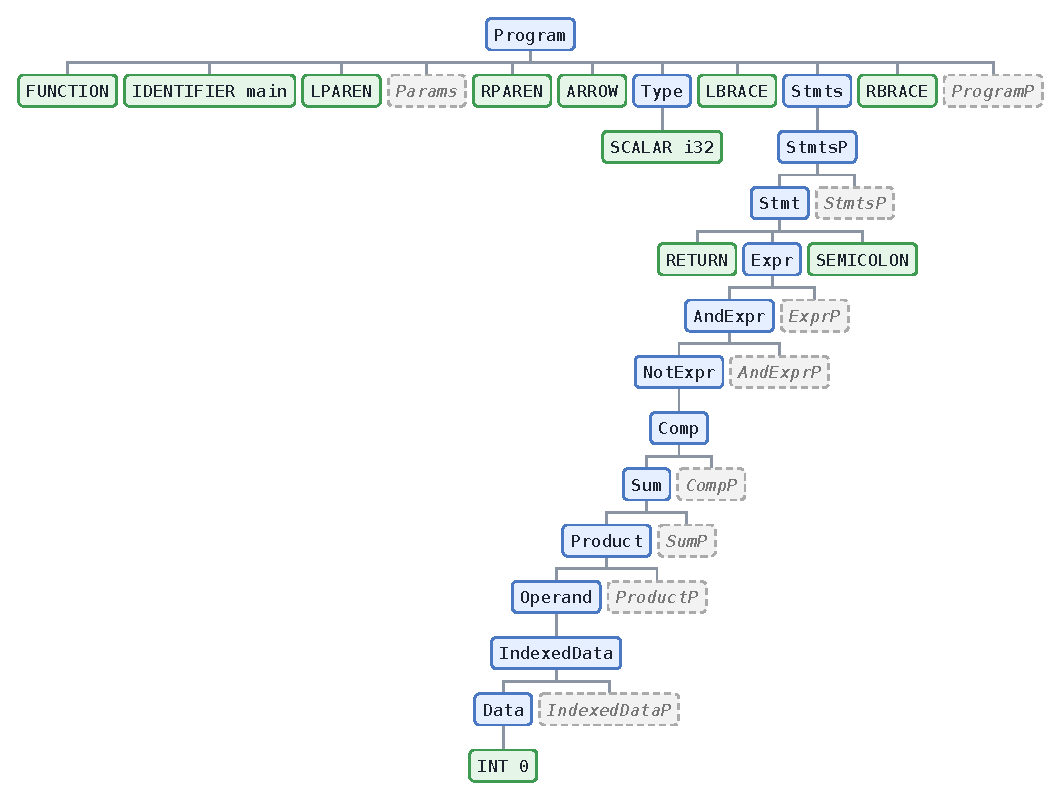
\includegraphics[width=0.8\linewidth]{resources/parse-tree-return0.pdf}
\caption{The parse tree of the minimal program.}
\label{fig:tree-tiny}
\end{figure}

\subsection{Operator Precedence}

The next example shows the precedence chain actually branching, rather
than passing straight through:

\begin{lstlisting}[caption={A declaration whose initializer branches.},
    label=lst:precedence-example]
function foo() -> i32 {
    i32 x = 1 + 2 * 3;
}
\end{lstlisting}

Figure~\ref{fig:tree-expr} draws its tree. The addition is the outer
operation: \nt{Sum} holds the \code{1}, and its \nt{SumP} child holds the
\code{+} together with the \nt{Product} for \code{2 * 3}, which is where
the multiplication is parsed, one level further down, before the addition
around it is complete. This is precedence shown structurally, with no
parentheses needed to force the multiplication to bind tighter.

\begin{figure}[H]
\centering
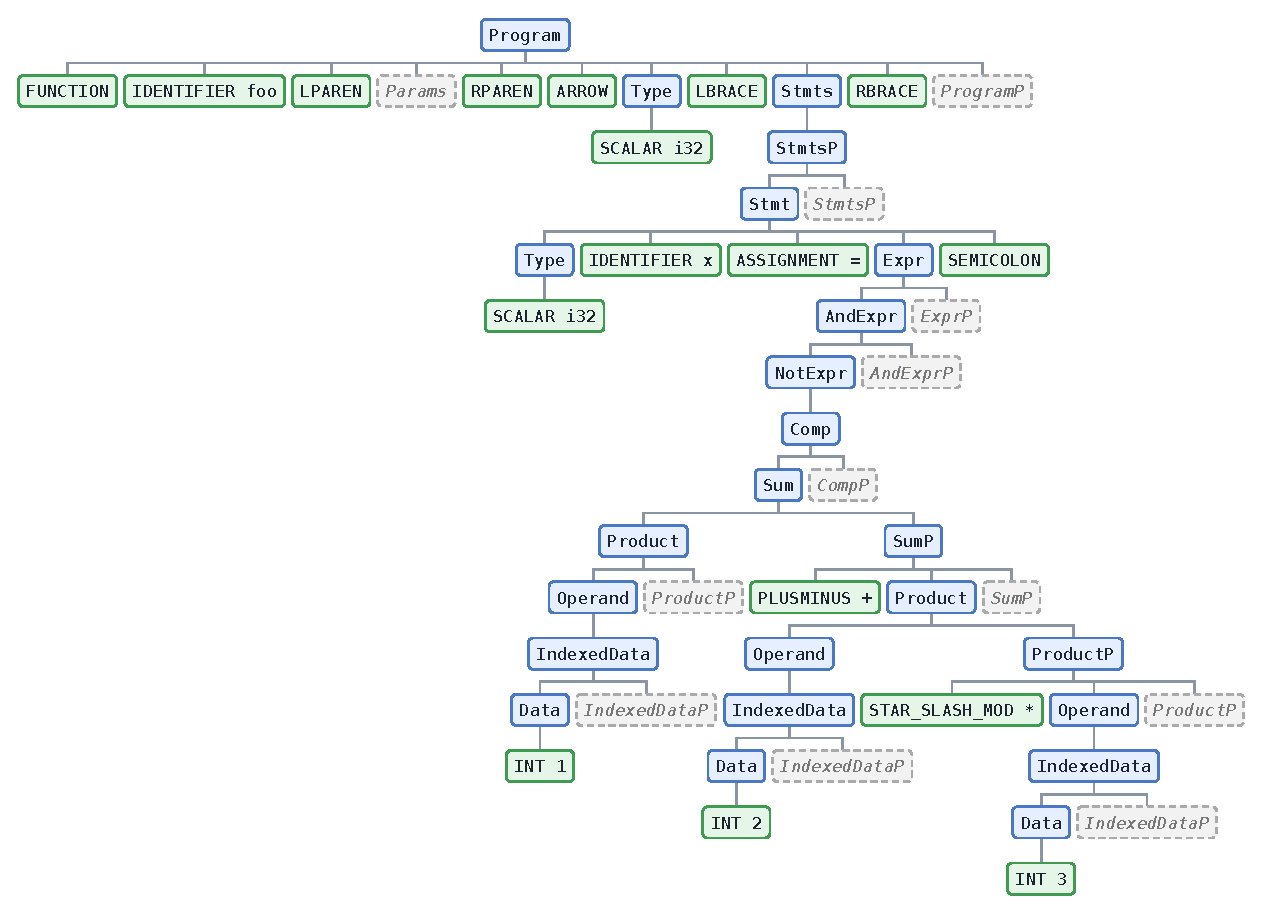
\includegraphics[width=\linewidth]{resources/parse-tree-expr.pdf}
\caption{The parse tree of Listing~\ref{lst:precedence-example}.}
\label{fig:tree-expr}
\end{figure}

In both figures, a nonterminal node is blue, a token is green, and a
nonterminal that derived the empty string is grey and dashed. Most of the
grey around the edges of Figures~\ref{fig:tree-tiny} and~\ref{fig:tree-expr}
is exactly this: nearly every \nt{...P} nonterminal in a short program
derives the empty string, since the recursion it stands for never runs for
more than a round or two.

\section{Parsers in the Real World}

The parser of OctaC, like its lexer, is hand-written rather than generated,
and deliberately small. This section looks at how parsers are built in
practice, and which simplifications ours makes.

\subsection{Parser Generators and Parsing Methods}

Many parsers are produced by a generator, the same way many lexers are.
Bison, upward compatible with the older Yacc, converts a grammar annotated
with actions into a parser, using LALR(1) tables by default
\cite{bison-manual}. LALR is a bottom-up method that accepts a larger class
of grammars than LL(1), at the cost of a less direct relationship between
the grammar and the code that results \cite{aho2006compilers}.

OctaC's grammar is restricted to LL(1) on purpose, so that the parser can
be a direct, hand-written translation of it, with no generated code and no
table beyond the one a human reads from the grammar itself.

\subsection{Hand-Written Recursive Descent}

Recursive descent is also a common choice for production compilers, not
only a teaching technique. Clang's parser is hand-written recursive
descent over the grammar of C and C++ \cite{clang-internals}, and CPython's
parser has been a hand-written PEG parser, a close relative of recursive
descent with unlimited lookahead and backtracking, since Python 3.9
\cite{python-pep617}. A hand-written parser gives the same advantages a
hand-written lexer does: direct control over error messages and recovery,
and no dependency on a generator as part of the build.

\subsection{Error Recovery}

Real parsers recover from a syntax error so that one run can report more
than the first one found, the same reason ours does. The general strategy,
skipping input until a token is reached that the grammar allows at some
enclosing point, is called panic mode recovery \cite{aho2006compilers}.
OctaC's parser is a direct application of it, with exactly two recovery
points chosen for the shape of the grammar: the end of a statement, and
the start of a function.

\subsection{Simplifications in OctaC}

Table~\ref{tab:parser-simplifications} summarizes the differences.

\begin{table}[H]
\centering
\small
\renewcommand{\arraystretch}{1.15}
\begin{tabular}{@{}>{\raggedright\arraybackslash}p{70pt}>{\raggedright\arraybackslash}p{190pt}>{\raggedright\arraybackslash}p{172pt}@{}}
\toprule
\textbf{Concern} & \textbf{Real-world parsers} & \textbf{OctaC} \\
\midrule
Construction & Generated from a grammar, or hand-written \cite{bison-manual,clang-internals} & Hand-written recursive descent \\
Grammar class & LALR or PEG, each more permissive than LL(1) \cite{aho2006compilers,python-pep617} & LL(1), by construction \\
Lookahead & Unbounded, with backtracking in a PEG parser \cite{python-pep617} & Exactly one token, never backtracks \\
Error recovery & Panic mode, or finer-grained strategies tuned per construct \cite{aho2006compilers} & Panic mode, at two recovery points \\
Tree & Often folded into an AST during parsing & A literal parse tree, one node per grammar symbol \\
Ambiguity & Resolved by precedence declarations in the generator & Resolved in the grammar itself, by construction \\
\bottomrule
\end{tabular}
\caption{Real-world parsers compared with the OctaC parser.}
\label{tab:parser-simplifications}
\end{table}
